\chapter{Podłoże teoretyczne}
\label{c3}

\section{Wstęp}
\label{c31}
Kolejny rozdział przedstawia aktualne metody i istniejące algorytmy związane z tematem pracy. Poza podstawowym algorytmem Apriori (\cite{Agrawal}), który używa drzew haszowych do przechowywania kandydatów, opisano trzy modyfikacje tego algorytmu. Główna różnica polega na tym, że wykorzystują one inną strukturę, a mianowicie drzewa prefiksowe. Są to rozwiązania zaproponowane przez Christina Borgelta (\cite{Borgelt}), Ferenca Bodona (\cite{Bodon}) oraz Barta Goethalsa (\cite{Goethals}). Ze względu na wykorzystanie prostszej struktury okazały się one szybsze od standardowego algorytmu.
 
Innym problemem jest optymalizacja wykonania kilku zadań Apriori uruchomionych współbieżnie na nakładających się podzbiorach tabeli z danymi. Metody z tym związane to Common Counting (\cite{WojciechowskiCC}) i Common Candidate Tree (\cite{WojciechowskiCCT}). Oparte są one o implementację Apriori z zastosowaniem drzew haszowych. Brakuje jednak adaptacji tych algorytmów, polegającej na zmianie struktury na drzewa prefiksowe. Właśnie taka modyfikacja została wprowadzona, a uzyskane efekty opisano w kolejnych rozdziałach niniejszej pracy. 


\section{Przegląd istniejących rozwiązań}
\label{c32}

\subsection{Algorytm Apriori \cite{Agrawal}}
\label{c321}
Algorytm Apriori jest algorytmem eksploracji poziomej. Szuka zbiorów częstych o rozmiarach \(1, 2,\dots , k\). Algorytm rozpoczyna od zbiorów o rozmiarze 1 i następnie zwiększa ten rozmiar w kolejnych iteracjach. Elementy każdej transakcji są uporządkowane leksykograficznie - jeżeli nawet transakcje nie są posortowane, to krokiem wstępnym algorytmu może być leksykograficzne uporządkowanie elementów transakcji (\cite{Morzy}). Po pierwszym kroku zebrane są zatem wszystkie elementy występujące w transakcjach (w postaci zbiorów jednoelementowych). Następnie sprawdzane jest, które z nich posiadają wsparcie nie mniejsze niż \(minsup\). Elementy niespełniające tego wymagania są odrzucane. Pozostałe służą do utworzenia dwuelementowych zbiorów kandydujących (ang. \textit{candidate itemsets}). Dla wygenerowanych zbiorów sprawdzane jest czy posiadają wsparcie równe co najmniej \(minsup\). Jeśli tak, to taki zbiór jest dodawany do listy zbiorów częstych i w kolejnej iteracji jest wykorzystywany (wraz z innymi zbiorami z tejże listy) do generowania zbiorów kandydatów o rozmiarze o 1 większym. Wsparcie zbiorów sprawdzane jest na podstawie odczytu danych z bazy danych. Algorytm zatrzymuje się gdy nie ma już możliwości generowania kolejnych zbiorów. W wyniku jego działania zwracana jest suma \(k\)-elementowych zbiorów częstych \((k = 1, 2,\dots)\), która może zostać wykorzystana do generowania reguł asocjacyjnych.

\subsection{Algorytm Apriori - implementacja Christina Borgelta \cite{Borgelt}}
\label{c322}
W tym podrozdziale opisany została adaptacja algorytmu Apriori autorstwa Borgelta. Odstępstwo od oryginału polega przede wszystkim na zmianie struktury, czyli wykorzystaniu drzew prefiksowych zamiast drzew haszowych. Rysunek 3.1 przedstawia taką właśnie strukturę. 
\begin{figure}[h]
\centering
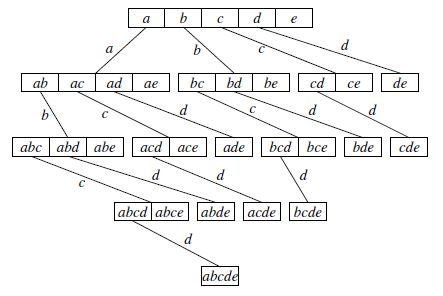
\includegraphics[width=0.8\linewidth]{figures/prefixTreeBorgelt}
\caption[Rysunek 3.1]{Drzewo prefiksowe dla 5 elementów (puste zbiory nie zostały zaprezentowane).}
\label{fig:prefixTreeBorgelt}
\end{figure}
Drzewo budowane jest od korzenia do liści (ang. \textit{top-down}), przy sprawdzaniu czy dana gałąź może zawierać zbiory częste. Jeśli ten warunek nie jest spełniony, to następuje odcięcie i ta część drzewa nie jest dalej generowana ani analizowana, gdyż nie zawiera przypadków, które powinny zostać uwzględnione w wynikach działania algorytmu. 

\subsubsection*{Struktura wierzchołka}
Wierzchołki drzewa prefiksowego reprezentowane mogą być na 3 sposoby:\newline
-- jako proste wektory liczb całkowitych (w tym przypadku następuje niejawne powiązanie każdego z możliwych elementów z pojedynczym polem wektora)\newline
-- jako wektory przechowujące licznik wystąpień wraz z identyfikatorem elementu\newline
-- jako drzewa haszowe wiążące dany element z licznikiem jego wystąpień

W pierwszym przypadku plusem jest to, że nie potrzeba pamięci na składowanie identyfikatorów elementów oraz fakt szybkiego dostępu do licznika. Minusem jest z kolei problem powstawania dziur w wektorze, tzn. wektor uwzględnia również informacje o licznikach elementów, o których wiadomo (na podstawie wcześniejszych iteracji), że nie mogą być częste. Jest to najlepszy wybór w przypadku, gdy priorytetem jest szybkość wykonania.

Druga struktura pozwala niwelować wyżej opisany problem i przechowuje jedynie te liczniki, które są nadal potrzebne. Minusem jest natomiast fakt zapotrzebowania na dodatkową pamięć na przechowywanie identyfikatorów oraz wolniejszy dostęp spowodowany koniecznością wyszukania licznika powiązanego z danym elementem. Mimo to jeśli optymalizacja pod kątem użycia pamięci jest istotniejsza od szybkości wykonania, to ta właśnie struktura powinna zostać wykorzystana.

Trzecia propozycja daje możliwość szybkiego dostępu do licznika, ale wymaga większej ilości pamięci. Jednakże to rozwiązanie nie daje łatwej możliwości sortowania elementów, dlatego też zostało odrzucona przez Borgelta.

\subsubsection*{Reprezentacja elementu}
Reprezentacja elementu ma duży wpływ na wspomniany wcześniej problem powstawania dziur w wektorze. Jeśli elementy są kodowane jako liczby całkowite, to jest to korzystne dla ograniczenia liczby i wielkości dziur. W przeciwnym razie problem ten może się nasilać. Dla dodatkowego zmniejszenia występowania tego problemu stosuje się podejście heurystyczne polegające na posortowaniu elementów malejąco względem częstości ich występowania i nadaniu elementom o podobnej liczbie wystąpień takiego samego identyfikatora (przy równoczesnym odrzuceniu tych, które występują mniej razy niż wynosi \(minsup\)). 

\subsubsection*{Przetwarzanie transakcji}
Struktura drzewa prefiksowego pozwala na proste przetwarzanie transakcji, w których elementy są posortowane. Dla poszczególnych wierzchołków odbywa się to rekurencyjnie i przebiega w następujący sposób: (1) idź do dziecka odpowiadającego pierwszemu elementowi w transakcji i przetwarzaj kolejne elementy rekurencyjnie dla tego dziecka i (2) usuń pierwszy element z transakcji i przetwarzaj dla danego wierzchołka. Krok 1 może zostać zakończony w momencie osiągnięcia poziomu drzewa, dla którego testowane są zbiory kandydatów. Wówczas algorytm nie przechodzi dalej do dziecka, nawet jeśli istnieją kolejne elementy w transakcji. 

Dzięki posortowaniu elementów można dodatkowo zoptymalizować działanie algorytmu. Po pierwsze można opuścić analizę elementów mających niższy identyfikator niż ten w przetwarzanym wierzchołku. Po drugie w przypadku gdy pierwszy element ma wyższy identyfikator niż ostatni element w wierzchołku, to można zrezygnować z rekurencyjnego przetwarzania danej transakcji dla wierzchołka. Dodatkowo jeśli elementów transakcji jest mniej niż zawierają wierzchołki na aktualnie analizowanym poziomie, to można zakończyć rekurencję, gdyż pożądany poziom drzewa nie zostanie osiągnięty.

Najłatwiej jest przetwarzać transakcje stosując wyżej opisaną metodę. Jednakże ze względu na wysoki koszt operacji rekurencyjnych możliwe są pewne ulepszenia. Jednym z nich jest pogrupowanie podobnych transakcji i umieszczenie ich w drzewie prefiksowym. Mogą być one przetwarzane wspólnie, ale należy mieć na uwadze, aby zyski były większe niż koszty stworzenia takich drzew i odpowiedniego przypisania do nich transakcji. 

Kolejnym zabiegiem usprawniającym wykonanie algorytmu jest usuwanie z transakcji elementów, które nie wchodzą w skład wierzchołków na poziomie \(k-1\) (gdzie \(k\) to liczba elementów w wierzchołkach aktualnie analizowanego poziomu drzewa). Zmniejsza to rozmiar transakcji i liczbę wywołań rekurencyjnych, ale trzeba pamiętać, że w przypadku zastosowania drzew prefiksowych do grupowania transakcji wymagana jest kosztowna operacja przebudowania tychże drzew.

Algorytm działa szybciej niż oryginalny Apriori, a wybór struktury wierzchołka i wybranych optymalizacji zależy głównie od badanego zbioru danych. 

\subsection{Algorytm Apriori - implementacja Ferenca Bodona \cite{Bodon}}
\label{c323}
W tej sekcji opisana została modyfikacja algorytmu Apriori zaproponowana przez Ferenca Bodona. Podobnie jak w przypadku wyżej opisanej implementacji Borgelta (\cite{Borgelt}) zastosowano strukturę drzewa prefiksowego oraz kilka dodatkowych optymalizacji opisanych poniżej. 

\subsubsection*{Struktura drzewa}
Drzewo budowane jest wierzchołka, który znajduje się na głębokości 0. Jest ono skierowane w dół, tzn. wierzchołki na poziomie \(d\) wskazują na wierzchołki na poziomie \(d + 1\). Krawędzie drzewa są oznaczone, a ich etykiety odpowiadają elementom transakcji, natomiast w wierzchołkach umieszczony jest identyfikator wierzchołka. Przykładowe drzewo zostało przedstawione na rysunku 3.2. 
\begin{figure}[h]
	\centering
	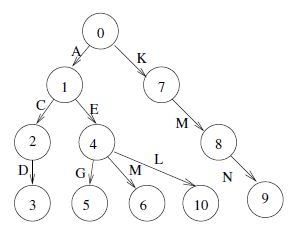
\includegraphics[width=0.5\linewidth]{figures/prefixTreeBodon}
	\caption[Rysunek 3.2]{Przykładowe drzewo prefiksowe dla 5 kandydatów \(\{A,C,D\}\), \(\{A,E,G\}\), \(\{A,E,L\}\), \(\{A,E,M\}\), \(\{K,M,N\}\).}
	\label{fig:prefixTreeBodon}
\end{figure}
W drzewie składowani są kandydaci (wraz z licznikami wystąpień), a także zbiory częste. Pozwala to na łatwe i szybkie generowanie kandydatów. Transakcje przetwarzane są sekwencyjnie i dla każdej transakcji \(t\) wyznaczany jest zbiór \(X\) \(k\)-elementowych (posortowanych) podzbiorów \(t\), gdzie \(k\) to rozmiar aktualnie szukanych kandydatów. Jednakże dąży się do niegenerowania wszystkich możliwych podzbiorów i jak najwcześniejszych wycofań. W momencie odnalezienia \(X\) w drzewie inkrementuje się licznik dla danego kandydata i kontynuuje przetwarzanie w głąb drzewa tylko jeśli algorytm znajduje się na głębokości \(d\), po przejściu krawędzią z etykietą \(j\), istnieje krawędź wychodząca oznaczona etykietą~\(i\), taką że \(i\in t\) oraz \(i < |t| - k + d + 1\). Również odnajdywanie reguł asocjacyjnych jest szybsze. Wynika to bezpośrednio z faktu, że - dzięki wykorzystaniu drzewa prefiksowego - obliczanie wsparcie zbiorów elementów jest wydajniejsze. Kolejnym plusem jest łatwiejsza implementacja co przekłada się na łatwiejszy w utrzymaniu kod.  

\subsection*{Metody obliczania wsparcia}
Wsparcie jest obliczane poprzez sekwencyjną analizę transakcji i ustalanie czy którzy kandydaci znajdują się w danej transakcji \(t\), a którzy nie. Jest to kosztowna operacja powtarzana i determinuje ona czas wykonania całego algorytmu. Może być wykonana na dwa sposoby. Oba startują z korzenia drzewa i opierają się na rekurencji. Pierwszy z nich dla każdego elementu \(t\) sprawdza czy istnieje krawędź a etykietą odpowiadającą elementowi. Sprowadza się to do wyszukiwania w posortowanym zbiorze. Druga metoda operuje na dwóch iteratorach - pierwszy z nich iteruje po elementach \(t\), drugi po krawędziach wierzchołka. Oba rozpoczynają iterację w pierwszym elemencie (odpowiednio transakcji i drzewa) i jeśli wskazują na ten sam element, to oba przechodzą do dalszej analizy. W przeciwnym wypadku iterator wskazujący na niższy element jest zwiększany. Przetwarzanie kończy się gdy jeden z iteratorów osiągnie odpowiednio koniec transakcji lub ostatnią gałąź.

Obie metody są poprawne, a różnica polega w sposobie wywołań rekurencyjnych. Dla pierwszej metody liczą kroków potrzebna do wykonania z poziomu wierzchołka o \(m\) krawędziach wychodzących odpowiada \(min\{|t| log_2{m},\nolinebreak m\nolinebreak log_2{|t|}\}\), dla drugiej mieści się w przedziale \(<min\{m,\nolinebreak|t|\},\nolinebreak m\nolinebreak+\nolinebreak|t|>\). W testach przeprowadzonych przez Bodona (\cite{Bodon}) druga metoda okazała się średnio dwukrotnie szybsza i to ona została wykorzystana do dalszych rozważań.

\subsection*{Modyfikacje optymalizujące czas wykonania}
W (\cite{Bodon}) zaproponowano kilka zabiegów optymalizujących czas wykonania algorytmu. Skupiają się one przede wszystkim na skróceniu czasu potrzebnego na obliczanie wsparcia kandydatów. Z reguły wymagają więcej pamięci, aby składować dodatkowe informacje, ale mimo to w ostatecznym rozrachunku są opłacane. Zostały one przedstawione w poniżej.

Pierwszy z nich polega na składowaniu długości maksymalnej ścieżki. Dla każdego wierzchołka pamiętana jest długość najdłużej ścieżki (począwszy od tego wierzchołka). Dzięki temu w momencie gdy wiadomo, że nie ma możliwości znalezienia w danej gałęzi kandydatów o zadanej długości jest ona pomijana. Zmniejsza to liczbę odwiedzanych wierzchołków i znacznie skraca czas poszukiwania dużych zbiorów elementów - co zostało potwierdzone doświadczalnie.

Kolejny zabieg polega na wykorzystaniu częstotliwości występowania elementów i przechowywaniu jej (oraz jej odwrotności) wraz z elementami oraz reorganizacji drzewa względem tej właśnie wartości (rysunek 3.3). Wówczas szukając wierzchołków reprezentujących zadany zbiór elementów stosowane jest wyszukiwanie liniowe a nie binarne. Dzięki wyżej wspomnianemu posortowaniu szybciej znajdowane są elementy występujące często, ale to do nich jest najwięcej odwołań, więc jest to pożądany efekt. Dodatkowo przeorganizowane drzewo nie jest zbalansowane, a to skutkuje tym, że jest mniej krawędzi do przejścia, co przekłada się bezpośrednio na mniej kosztownych wywołań rekurencyjnych. Zastosowanie tej modyfikacji skutkuje zwiększonym czasem generowania kandydatów, ale pozwala na szybsze obliczenie wsparcia kandydatów. Jako, że druga operacja jest bardziej kosztowna, to jest to zabieg opłacalny.
\begin{figure}[h]
	\centering
	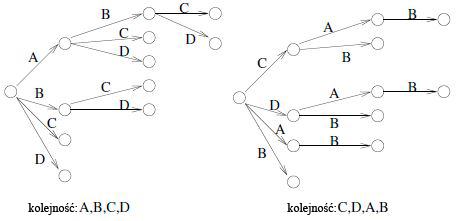
\includegraphics[width=0.8\linewidth]{figures/reorderedTreeBodon}
	\caption[Rysunek 3.3]{Zmieniona organizacja drzewa prefiksowego dla dwóch 3-elementowych kandydatów \(\{A, B, C\}\), \(\{A, B, D\}\)}
	\label{fig:reorderedTreeBodon}
\end{figure}


Wsparcie zbiorów jedno- i dwuelementowych może być obliczane w szybszy sposób niż za pomocą opisywanego drzewa. Dla przyspieszenia wykonania zalecane jest wykorzystanie wektora (dla jednoelementowych) lub tablicy dwuwymiarowej (dla dwuelementowych). Daje to możliwość łatwego dostępu do poszczególnych kandydatów i ich licznika, a także jest mniej wymagające pamięciowo. 

Następna modyfikacja polega na zastosowaniu technik haszujących. Sprowadza się to do zmiany reprezentacji krawędzi wychodzących z danego wierzchołka z posortowanej listy na tablicę haszujacą. Pozwala to przyspieszyć przeszukiwanie drzewa, a co za tym idzie liczenie wsparcia. Jednakże drzewa haszowe są znacznie bardziej wymagające pamięciowo. Dlatego też powinno stosować się je gdy liczba krawędzi wychodzących przekracza pewną ustaloną wartość. W wyniku tego założenia otrzymane drzewo będzie miało tablice haszowe jedynie do pewnego momentu, potem struktura wierzchołka pozostanie niezmieniona. Dzięki temu tam gdzie przeszukiwanie było wolne zostanie ono przyspieszone, a tam gdzie - ze względu na małą ilość krawędzi - było szybkie, nadal będzie szybkie. 

Kolejna zmiana zaproponowana w \cite{Bodon} odnosi się do Dzielnego Apriori (ang. \textit{Apriori-Brave}). Jest to heurystyka wykorzystująca śledzenie użycia pamięci. Polega na generowaniu kandydatów o rozmiarach \(k\nolinebreak+\nolinebreak 1, k\nolinebreak+\nolinebreak 2, \dots\) (\(k\) - rozmiar największych znalezionych zbiorów częstych) bez sprawdzania wsparcia tych kandydatów do momentu aż wymagana będzie cała dostępna pamięć. Prowadzi to do redukcji odczytów wszystkich transakcji z bazy danych, ale skutkuje także generowaniem fałszywych kandydatów, dla których również obliczane musi być wsparcie. Dlatego też metoda ta nie gwarantuje zysków względem oryginalnego Apriori, ale - jak wykazały testy - heurystyka ta sprawdza się w praktyce.

Ostatnią modyfikacją jest usunięcie z transakcji niepotrzebnych elementów. Po pierwszym odczycie całej bazy wiadomo, które elementy są częste, a które nie. Mając na uwadze własność anty-monotoniczności miary wsparcia (\cite{Morzy}) można ze wszystkich transakcji usunąć elementy nieczęste, gdyż nie wpłynie to na wynik działania algorytmu, a pozwoli zmniejszyć liczbę kroków wykonania. 

\subsection{Algorytm Apriori - implementacja Barta Goethalsa \cite{Goethals}}
\label{c324}
W poniżej sekcji omówiono implementację algorytmu Apriori przedstawioną przez Goethalsa. Podobnie jak w uprzednio opisanych adaptacjach tego algorytmu,  w miejsce drzewa haszowego, wykorzystana została struktura drzewa prefiksowego. Głównym elementem, który został poprawiony jest liczba odczytów bazy danych. Jej zredukowanie przekłada się bezpośrednio na czas wykonania algorytmu. Do osiągnięcia takiego efektu wykorzystana została idea górnych ograniczeń (ang.\textit{upper bound}), które zostały opisane poniżej.

\subsection*{Górne ograniczenie na liczbę zbiorów kandydatów}
Zastosowanie górnych ograniczeń wymaga znalezienia odpowiedzi na pytanie (przy założeniu, że znane są numer obecnej iteracji oraz kolekcja zbiorów częstych na tym poziomie wykonania algorytmu): ile maksymalnie kandydatów może zostać wygenerowanych w pozostałych iteracjach? Taka informacja pozwala na podjęcie dalszych odpowiednich kroków optymalizacyjnych. Goethals \cite{Goethals} zaproponował obliczanie górnej granicy na koniec każdej iteracji Apriori. Do ustalenia podstawowej górnej granicy wykorzystywany jest zbiór \(L\) zawierający ze wszystkie możliwe \(k\)-elementowe podzbiory. Zadanie to nie jest trywialne i zostało wsparte wieloma teoriami, które zostały potem potwierdzone eksperymentalnie. Wyniki tych eksperymentów pokazały, że możliwe jest ustalenie górnych granic w czasie zależnym liniowo od liczby obecnie odkrytych zbiorów częstych. Zredukowało to liczbę odczytów bazy danych przy jednoczesnym zysku pamięciowym związanym ze zmniejszoną liczbą generowanych kandydatów. 


\subsection{Common Counting (CC) \cite{WojciechowskiCC}}
\label{c325}
Często przeszukiwane zbiory danych służące do generowania reguł asocjacyjnych są bardzo liczne. Niejednokrotnie poszukiwane są reguły odnoszące się tylko do podzbioru tych danych. Wówczas należy sformułować odpowiednie zapytania eksploracyjne filtrujące dane w zadany sposób. Do optymalizacji zbioru takich zapytań służy algorytm Common Counting. W metodzie chodzi o równoległe wykonanie zbioru zapytań eksploracyjnych algorytmem Apriori z integracją porywających się fragmentów bazy danych. Na wejściu algorytm otrzymuje zbiór elementarnych predykatów selekcji danych dla zbioru zapytań eksploracyjnych \(DMQ\). Początkowo algorytm ustala zbiór wszystkich elementów, czyli takich, które wystąpiły w co najmniej jednej transakcji. W kolejnych krokach generowane są zbiory częste oddzielnie dla każdego z zapytań. Przebiega to w taki sam sposób jak w przypadku standardowego algorytmu Apriori. Z każdym zapytaniem powiązane jest drzewo haszowe, w którym przechowywani są kandydaci. Warunek zatrzymania algorytmu jest taki jak w standardowym Apriori (brak możliwości wygenerowania kandydatów w kolejnej iteracji), z tą różnicą, że musi być spełniony dla wszystkich zapytań ze zbioru. 
Zliczenie wystąpień kandydatów jest realizowane dla wszystkich zapytań jednocześnie. Partycje bazy danych są odczytywane sekwencyjnie dla poszczególnych elementarnych predykatów selekcji danych. Powiększeniu ulegają liczniki kandydatów zawartych w analizowanej transakcji dla zapytań posiadających odwołania do danej partycji. Lista kandydatów zawierających się w danej transakcji ustalana jest poprzez testowanie transakcji względem drzew haszowych. Należy tutaj zaznaczyć, że w przypadku gdy kilka zapytań współdzieli dany elementarny predykat selekcji danych, to podczas zliczeń wystąpień kandydatów odczyt właściwej mu partycji jest wykonywany tylko raz. Zatem optymalizowane są odczyty współdzielonych przez zapytania fragmentów bazy danych, przy czym pozostałe kroki algorytmu Apriori pozostają niezmienione i są wykonywane oddzielnie dla każdego zapytania. 

\subsection{Common Candidate Tree (CCT) \cite{WojciechowskiCCT}}
\label{c326}
Common Candidate Tree jest podobnym algorytmem do Common Counting. Tak jak w przypadku CC algorytm przetwarza zbiór \(DMQ\) i zwraca zbiory częste dla poszczególnych jego elementów, a także korzysta z oryginalnego Apriori i wykorzystuje strukturę drzewa haszowego. Różnica polega na tym, że zwiększony został stopień współbieżności przetwarzania. Uzyskano to dzięki współdzieleniu pamięciowej struktury drzewa składującego kandydatów. Jest to duża zaleta w porównaniu z Common Counting, gdyż - zamiast wielu - tworzone jest jedno drzewo haszowe o niezmiennej strukturze. Poza zachowaniem integracji odczytów współdzielonych możliwa jest integracja testowania czy w danej transakcji zawierają się kandydaci z poszczególnych zapytań. Realizacja tego algorytmu wymagała rozszerzenia struktury kandydatów. W jej wyniku z każdym kandydatem związany został wektor liczników (jeden licznik dla jednego zapytania), a nie pojedynczy licznik. Dodatkowo - dla rozróżnienia zapytań, które wygenerowały danego kandydata - dołączony został wektor flag logicznych przechowujący taką właśnie informację. Po wyłonieniu kandydatów są oni umieszczani w jednym zbiorze. Zbiór ten trafia do wspólnego drzewa haszowego. W tym kroku modyfikowane są również odpowiednie flagi. Samo generowanie kandydatów i selekcja zbiorów częstych nadal realizowane są odrębnie dla poszczególnych zapytań. Zliczany jest natomiast zintegrowany zbiór kandydatów. Podczas tej fazy brani są pod uwagę tylko kandydaci wygenerowani przez zapytania odwołujące się do aktualnie odczytywanej partycji bazy danych i w przypadku gdy kandydat zawiera się w przetwarzanej transakcji, to zwiększa się liczniki kandydatów związane z tymi zapytaniami. Algorytm kończy się gdy nie można wygenerować kandydatów dla kolejnego poziomu drzewa. 

Eksperymenty \cite{WojciechowskiCCT} pokazały, że Common Candidate Tree jest wydajniejszy i lepiej skalowany od Common Counting.

\subsection{Podsumowanie}
\label{c327}
Przytoczone algorytmy są przykładami optymalizacji wykonania operacji znajdowania zbiorów częstych. Pierwsze trzy wykorzystują drzewa prefiksowe, a więc strukturę szybszą, prostszą i mniej wymagającą pamięciowo. Poza zmianą struktury stosowane jest sortowanie elementów transakcji według określonego dla danego algorytmu sposobu. Dwa ostatnie algorytmy (Common Counting i Common Candidate Tree) dokonują partycjonowania danych w celu zmniejszenia liczby operacji i sprawdzają się w sytuacji gdy należy wykonać wiele (przynajmniej częściowo nakładających się) zapytań eksploracyjnych odnoszących się do tego samego zbioru danych. Jednakże korzystają one z oryginalnej wersji algorytmu Apriori \cite{Agrawal}, a co za tym idzie ze struktury drzew haszowych, co skutkuje wolniejszym wykonaniem operacji generowania kandydatów i obliczania wsparcia, a także większych wymagań pamięciowych. W kolejnym rozdziale przedstawiono modyfikacje tych algorytmów. Zmiana polega właśnie na użyciu drzew prefiksowych i jednej z wcześniej opisanych adaptacji Apriori.